\documentclass[conference]{IEEEtran}
\IEEEoverridecommandlockouts
% The preceding line is only needed to identify funding in the first footnote. If that is unneeded, please comment it out.
\usepackage{cite}
\usepackage{amsmath,amssymb,amsfonts}
\usepackage{algorithmic}
\usepackage[vlined, ruled]{algorithm2e}
\usepackage{graphicx}
\usepackage{textcomp}
 \usepackage{makecell, diagbox, hhline, booktabs}
 \usepackage{url}

\def\BibTeX{{\rm B\kern-.05em{\sc i\kern-.025em b}\kern-.08em
    T\kern-.1667em\lower.7ex\hbox{E}\kern-.125emX}}

%~~~ Double-blind review macro ~~~~~~~~~~~~~~~~
\usepackage{lipsum}
\usepackage{xcolor}
\usepackage{soul}
\sethlcolor{black}
\makeatletter
\newif\if@blind
\@blindtrue %use \@blindfalse on final version
\if@blind \def\hl#1{}\else
   \let\hl\relax
\fi
%~~~~~~~~~~~~~~~~~~~~~~~~~~~~~~~~~~~~~~~~~~~

%~~~ Pseudocode comment formatting ~~~~~~~~~~~~
\newcommand\mycommfont[1]{\textcolor{blue}{#1}}
\SetCommentSty{mycommfont}
\DontPrintSemicolon 
%~~~~~~~~~~~~~~~~~~~~~~~~~~~~~~~~~~~~~~~~~~~


\begin{document}

\title{Cloud-assisted Control of Ground Vehicles using Adaptive Computation Offloading Techniques\\
%{\footnotesize \textsuperscript{*}Note: Sub-titles are not captured in Xplore and
%should not be used}
%\thanks{Identify applicable funding agency here. If none, delete this.}
}

% \author{\IEEEauthorblockN{Arun Adiththan}
% \IEEEauthorblockA{The City University of New York, New York, NY 10019\\
% Email: {\em arunadiththan@gmail.com}}
% \and
% \IEEEauthorblockN {Ramesh Sethu \& Soheil Samii}
% \IEEEauthorblockA{General Motors R\&D, Warren, MI 48090\\
% Email: {\em ramesh.s@gm.com}; ~{\em soheil.samii@gm.com}
% }}

% Double-blind review
\author{\IEEEauthorblockN{\hl{Arun Adiththan}}
\IEEEauthorblockA{\hl{The City University of New York, New York, NY 10019\\
Email: {\em arunadiththan@gmail.com}}}
\and
\IEEEauthorblockN {\hl{Ramesh Sethu \& Soheil Samii}}
\IEEEauthorblockA{\hl{General Motors R\&D, Warren, MI 48090\\
Email: {\em ramesh.s@gm.com}; ~{\em soheil.samii@gm.com}} \\
{\em Author names \& affiliation removed for the purpose of double-blind review}
}}


\maketitle

\begin{abstract}
{
\rm
The existing approaches to design efficient safety-critical control applications is constrained by limited in-vehicle sensing and computational capabilities. In the context of automated driving, we argue that there is a need to think {\em "out-of-the-vehicle"} to meet the sensing and powerful processing requirements of sophisticated algorithms (e.g., deep neural networks). The network data rate and bandwidth supported by the existing communication standards cannot adequately meet the hard-real-time requirements of core control computations. Therefore, it is important to identify parts of control computation that are amenable for offloading to the cloud (or edge)-based resources. We also need to develop mechanisms to handle network communication failure scenarios such as connectivity loss and large delays. To address the challenges, we propose an adaptive offloading technique for control computations into the cloud. The proposed approach considers both current network conditions and control application requirements to determine the feasibility of leveraging remote computation and storage resources. As a case study, we describe a cloud-hosted planning algorithm for a path following controller that is cognizant of dynamically changing road conditions using crowdsensed data. Our simulation results demonstrate improved controller performance in terms of distance and time, even in the presence of transient connectivity loss and large delays.	
}
\end{abstract}

% \begin{IEEEkeywords}
% component, formatting, style, styling, insert
% \end{IEEEkeywords}

\section{Introduction}
\label{sec:Introd.date17}
Modern cars increasingly rely on advances in information technology to offer safety-critical features to the users. Advanced driver-assistance systems (ADAS) help guide drivers and reduce accidents through various automated and adaptive features such as adaptive cruise control (ACC), autonomous emergency braking, and forward-collision warning. Such intelligent safety-critical aspects in vehicles are realized by running complex algorithms that process data obtained from several types of sensors such as RADAR, LIDAR, video camera, GPS, etc. The in-vehicle sense and computational capabilities have certain limitations such as sensing range and amount of energy required to perform compute-intensive tasks. The in-vehicle capabilities cannot be enhanced through additional hardware (such as duplicate sensors and powerful processors) beyond a certain limit after without increasing the system complexity and cost.

We posit that cloud computing technology can help address some of the existing limitations in terms of sensing and computation. Cloud computing allows users to acquire, scale up/down, and release computational and storage resources on-demand. Cloud resources can be treated as a utility (like electricity, for example) that can be accessed over Internet. Thus, cloud technology can be a suitable candidate to address the limitations of in-vehicle capabilities and enhance the functional and safety aspects of automotive control applications. Some of the major automakers offer several cloud-based non-control services like emergency scenario response such as remote unlocking, crash response, stolen vehicle tracking, battery health monitoring, and other diagnostic solutions.

We view cloud as a technology that not only offers an enhanced computational platform but also as an enriched information source (through means such as crowdsourcing). The enriched information essentially enhances the perception range of a vehicle by fusing together sensor data from multiple vehicles. In the context of offering advanced driver assistance features and autonomous driving, we envisage more and more automotive control applications involving cloud being developed in the future. Therefore, we think it is essential to explore various parts of automotive control application that benefit from and are feasible to be executed in the cloud. It is also necessary to develop techniques that are required to deal with potential failure scenarios so that the safety and stability of the control system is not compromised.

In this light, we have developed an offloading controller architecture that determines when it is feasible and beneficial to offload control computations, that may leverage additional data and computational resources, to the cloud. The proposed offloading approach is opportunistic and hence it is flexible to toggle between in-vehicle and cloud-based resources. We demonstrate the feasibility of our approach using a cloud-based path following controller case study in Matlab. The primitive waypoint generation algorithm for the controller is generated in cloud, leveraging crowdsourced data on current road conditions.  The network communication delays are modeled using NS-3 LTE library. Our results show improved performance of the path following controller in terms of both distance traveled by the vehicle and the time taken between a given source and destination.
\section{Adaptive Offloading Controller Design}
\label{sec:Off_Ctlr}
In this section, we present the computation offloading controller design for automotive control applications that leverages cloud. This approach enables dynamic switching between and on-board and remote resources based on the control application specification and current network conditions.

In the mobile cloud computing area, cloud-based augmentation techniques \cite{ref:MCC_aug, ref:cloudlet} and computation offloading problem \cite{ref:MCC_survey1, ref:MCC_survey2} have been extensively studied. However, major emphasis is placed on saving energy on mobile devices and computation offloading is largely determined by the viability of network conditions at any given point of time. In the automotive domain, however, the most important consideration is satisfying the real-time constraints of the control applications. A typical control loop in an application like adaptive cruise control (ACC) takes 10 ms. This, given the current network communication standards, makes it infeasible to offload core control computation to the cloud. Therefore, we need to identify parts of control computation that are amenable for offloading to the cloud without compromising on the safety and stability of the system. The candidate computational part must have a delay tolerance in the range of 150-200 ms and potentially benefit from additional computation resource and/or data accessed via cloud. 

\begin{figure}
%\hspace{0.2in}
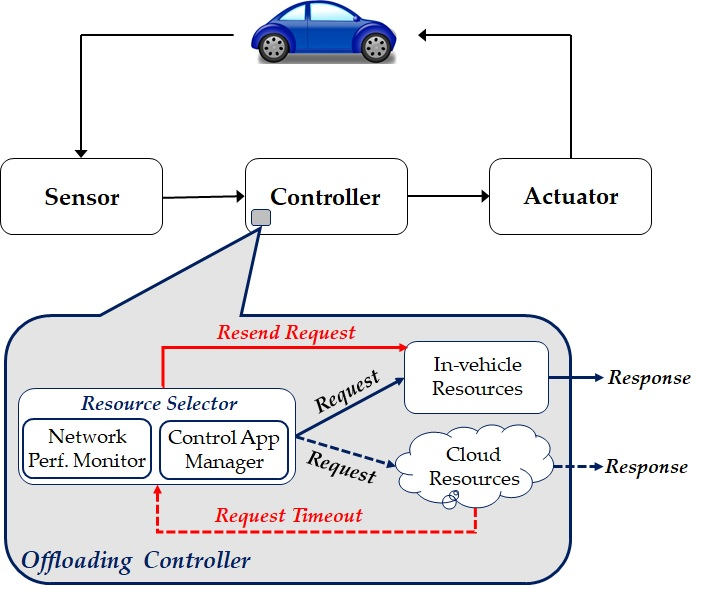
\includegraphics[width=3.25in,height=3in]{off_ctlr.jpg}
 \caption{Computation Offloading Controller Architecture \label{fig:OFF_CTLR}}
\end{figure}

Figure \ref{fig:OFF_CTLR} shows our offloading controller architecture design for control applications. The basic functionality of the offloading controller is to determine whether to execute a given computational task on local or remote resource. The decision-making process relies two components, namely, Network Performance Monitor and Control Application Specification. The network performance monitor component continuously monitors the network characteristics such as available bandwidth and uplink data rate. The control application specification component identifies the self-contained parts of control computation (e.g., pre-processing sensor data, vehicle state estimation) and their computational and latency requirements. These parts are specified as tasks and this task specification along with the current network conditions guide the process of selecting a resource. Once a suitable resource for a given task is identified, the task is executed on the resource and the response is fed to the control loop. 

\begin{algorithm}
\;
\tcc{Computation task ${T_{i}}$ = $(S_{i}, C_{i}, L_{i})$  where,\\
\hspace{0.3in}$S_{i}, S_{i}^{\prime}$: size of the input \& output data \\
\hspace{0.3in}$C_{i}$: \# of CPU cycles required for task  ${T_{i}}$ \\
\hspace{0.3in}$L_{i}$: latency requirement of the task ${T_{i}}$ \\
$C_{cloud}$: \# of CPU cycles available in the cloud \\
$\beta, \beta^{\prime}$: available uplink and downlink data rate \\
$T_{i}^{rsrc}$: resource to which the task {\em i} is assigned 
}
\;
 \SetKwInOut{Input}{Input}
 \SetKwInOut{Output}{Output}
\Input {Set of input tasks $\mathcal{T}=\{T_{i}\}, i=1,2,...,n$}
\Output {Task execution output: {$T_{i}^{out}$}}

\caption{Computation offloading: high-level steps}
\label{alg:off_ctlr}
\;
\begin{algorithmic}
\WHILE{$\mathcal{T} \neq $ NULL}
\STATE {\textbf{\underline{measure}}} available uplink data rate for task $T_{i}$: $\beta$
\STATE {\textbf{\underline{estimate}}} network delay: $\delta_{i}^{net}$ := $\frac{S_{i}}{\beta}$ + $\frac{S_{i}^{\prime}}{\beta^{\prime}}$
\STATE {\textbf{\underline{estimate}}} computation delay: $\delta_{i}^{comp}$  := $\frac{C_{i}}{C_{cloud}}$  \;
\IF {$\delta_{i}^{net}$+$\delta_{i}^{comp}$ $<$ $L_{i}$}
\STATE $T_{i}^{rsrc}$ := {\em cloud} 
\ELSE
\STATE $T_{i}^{rsrc}$ := {\em on-board} 
\ENDIF
\STATE {\textbf{\underline{execute}}} task on $T_{i}^{rsrc}$ and \textbf{return} $T_{i}^{out}$
\IF {$T_{i}^{rsrc}$ == cloud $\land$ timeout}
\STATE {\textbf{\underline{execute}}} task $T_{i}$ on {\em on-board} resource and \textbf{return} $T_{i}^{out}$
\ENDIF 
\ENDWHILE
\end{algorithmic}
\end{algorithm}

Algorithm \ref{alg:off_ctlr} describes the step-by-step process of resource selection and offloading. When the cloud resource is selected for task execution and the input data is offloaded to the cloud, the response might not come back within a desirable timeframe (say, for example, due to temporary resource outage). In such cases, the request timeout will get triggered and the same request will now have to be forwarded to the local resource. As pointed out in Section II, due to limited understanding of the surrounding context in the local-only case, the response generated by the local resource may be less efficient (in terms of time taken for task execution and/or the quality of control output) compared to a cloud-based approach. In the tradeoff analysis, particularly in a feedback control system in the automotive domain, the emphasis is more on the stability of the system than quality of output in one control step as compromising on stability could lead to undesirable consequences.
\section{Case Study: Cloud-based Path Following Controller}
\label{sec:case_study}
For communication latency modeling, we initially adopted an analytical model approach inspired from the Mobile Cloud Computing area. However, we realized that the analytical model approach was inadequate to capture the mobility aspects of the vehicles and lacks the ability to specify accurate communication link characteristics. So, we utilized the NS-3 LTE library \cite{ref:ns3_lte} to simulate the communication channel and measure latency using UDP application traffic. We had used the measured latency values in a path following control system in Matlab and studied the behavior of the system in different scenarios and under varying network conditions.

\subsection{Communication channel modeling using NS-3 LTE library}
\label{sec:ns3_lte}
The simulation setup in NS-3 includes one base station (aka eNB node) and constant velocity mobility model for the vehicles. Since we used LTE communication technology, we generated two distinct categories of traffic – one related to the control application and another video streaming traffic. The traffic flow in the former category is bidirectional whereas the entertainment traffic is unidirectional (from streaming servers to the end users in vehicles). The simulation setup is shown in Figure \ref{fig:NS3-SETUP}. 
\begin{figure}
%\hspace{0.2in}
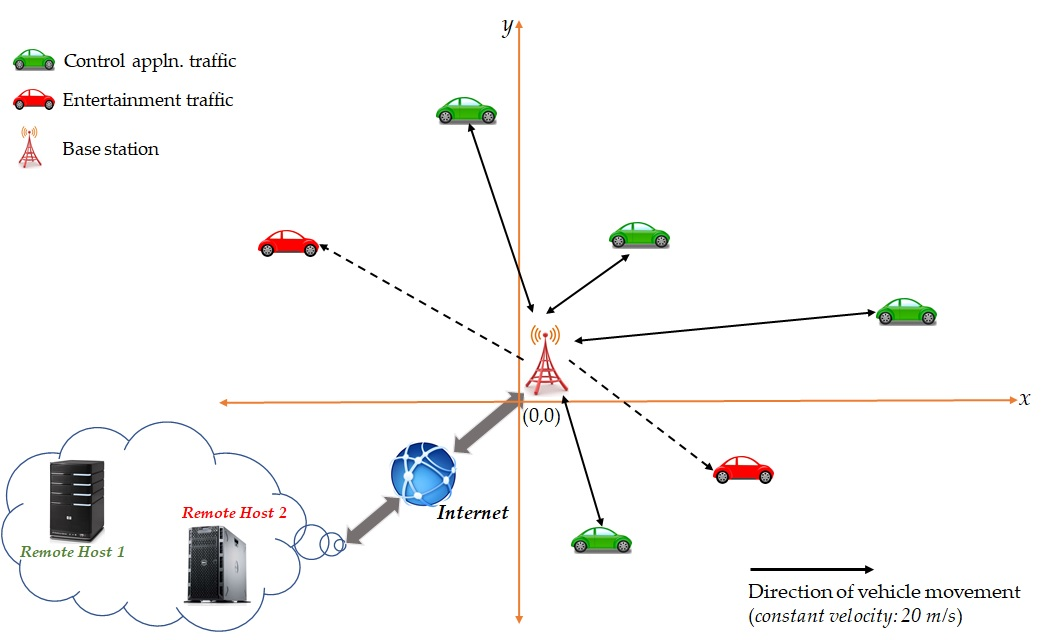
\includegraphics[width=3.5in,height=2.5in]{ns3_setup.jpg}
 \caption{Communication channel simulation setup  \label{fig:NS3-SETUP}}
\end{figure}

The downlink and uplink frequency bands of the cell are set to 2110 and 1710 MHz, respectively. The transmission power of the eNB node and the vehicle nodes is set to 40 and 20 dBm, respectively. In our simulation, Proportional Fair MAC Scheduler and Friis path loss model is used. The transmission method between the eNB node and vehicles is a single-hop unicast. Two distinct types of applications are configured on each remote host – an UDP Echo application on Remote Host 1 and a packet generator application on Remote Host 2. 

The control application traffic constitutes 80\% of the total traffic and the remaining 20\% is the entertainment traffic (1024 B packet every 20 ms). The packet size of the control application traffic transmitted by all but one vehicles is in the range of 128 to 2048 B every 20 ms. The remaining one vehicle, for which we are measuring the latency values, transmits 512 B packet every 20 ms. Table \ref{tab:ns3} shows the latency values obtained by varying number of vehicles and the network bandwidth. The latency values noted is an average of 10 runs for the vehicle the that transmits 512 B
packets every 20 ms. 

\begin{table}[ht]
\centering
\begin{tabular}{|l|c|c|c|c|c|}\hline
\theadfont\diagbox[width=11em]{{\bf Bandwidth}}{{\bf \# vehicles}}&
\thead{15}&\thead{30}&\thead{45}&\thead{60}&\thead{75}\\    \hline
5 MHz & 51.44 & 52.09  & 52.92 & 99.49  & 100.66\\
\hline
10 MHz & 37.28  & 42.01 & 42.1 & 68.49 & 89.38\\
\hline
\end{tabular}
\bigskip
\caption{Data transfer latency (ms)}
\label{tab:ns3}
\end{table} 

\subsection{Path following controller simulation in MATLAB}
\label{sec:matlab_sim}
We had chosen the pure pursuit controller algorithm that is available in the Robotic Systems Toolbox in Matlab \cite{ref:matlab_rst}. The sampling interval for the pure pursuit controller meets some of the offloading constraints specified in Section \ref{sec:Off_Ctlr} and hence determined as a suitable candidate to offload the computation to the cloud. 

The pure pursuit controller basically implements a path tracking algorithm that keeps track of and controls the robot’s movements along the path. The path between a source and destination is comprised of a set of waypoints (or intermediate [x y] coordinates). The fundamental operation in the controller is the computation of linear and angular velocities for the next control step based on the current pose of the robot. The pose is specified as [x, y, theta], where (x, y) represents a point in the reference coordinate system and “theta” represents the heading angle of the robot. 

In this work, we have extended the static waypoint generation and path following controller code (in \cite{ref:matlab_rst}) to dynamically generate waypoints using purely on-board or remote cloud resources. The other contribution is the simulation of failure scenarios such as network connectivity loss and large delays and demonstrate switching between local and cloud resources for waypoint generation. The cloud-based waypoint generation factors in the most up-to-date information about the constantly changing road conditions and hence can compute a more efficient path for the robot. 

In our work, we adopt a primitive approach for waypoint generation. We assume that the robot is operating in an environment where from any given point, there are three potential directions – namely, vertical, horizontal, or diagonal -- the robot can move on. Each potential direction has a weight associated with it that captures the “quality” of the path (e.g., if a path has a pothole or stalled traffic, it will have less weight and hence deemed as a low-quality path). The primitive waypoint generation algorithm always picks the path with the highest quality. In the local-only waypoint generation approach we assume that the weights remain static or change at much lower frequency compared to cloud (due to the large overhead incurred in V2V communication, for example). Therefore, the local-only approach might yield a path between source and destination that incurs larger distance, more time, or both. 

The first set of results shown in Figure \ref{fig:PF_A_B} demonstrates the differences in path computed fully on-board (a) and upfront (without factoring in changes in the road conditions) and path computed fully in the cloud (b) that dynamically adjusts weights based on crowdsourced data. We can see that the fully remotely computed path incurs less distance and time. The noted time values are adjusted by multiplying it with the path weight. For the cloud computation part, we have used the communication latency values obtained for N=30 vehicle case in the NS-3 simulation.

\begin{figure}
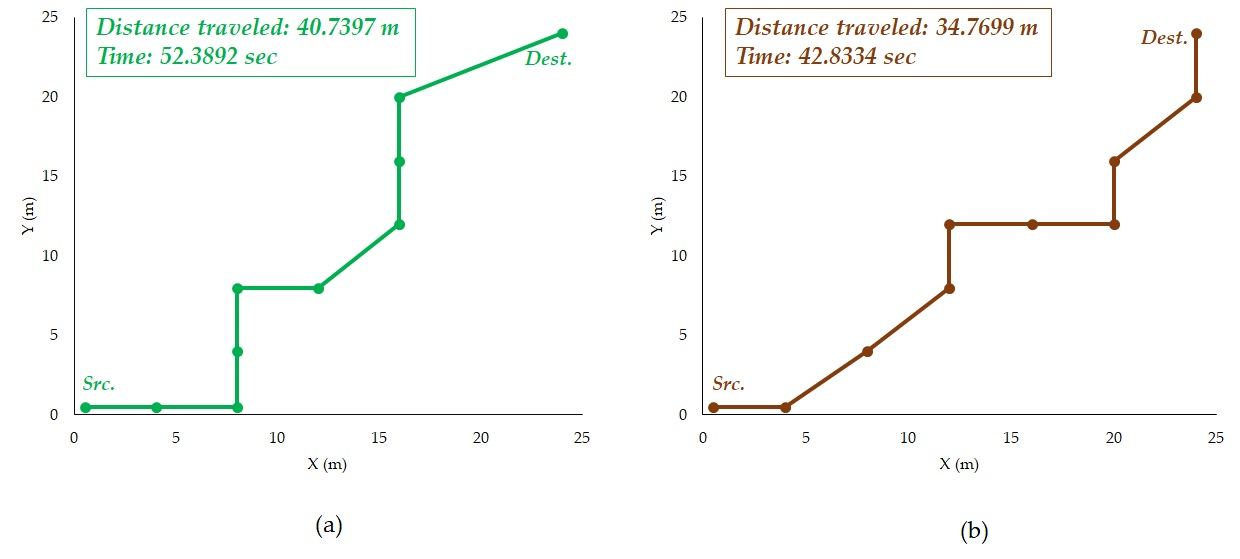
\includegraphics[width=3.5in,height=2.5in]{pf_a_b.jpg}
 \caption{Waypoint generation: (a) fully on-board without factoring in dynamically changing road conditions; (b) fully in the cloud using up-to-date data on current road conditions  \label{fig:PF_A_B}}
\end{figure}

The second set of results shown in Figure \ref{fig:PF_C} highlight the switching between local and remote resources in the presence of a network communication failure. It shows the impact of connectivity loss to the cloud server. When the connectivity loss is detected by the Network Performance Monitor component of the offloading controller (c.f.: Figure \ref{fig:OFF_CTLR}), the resource selector component chooses to leverage local resources for the next waypoint generation. Since the local knowledge is either static (or less frequently updated) compared to cloud, it results in a less efficient path than a purely cloud-based approach.

\begin{figure}
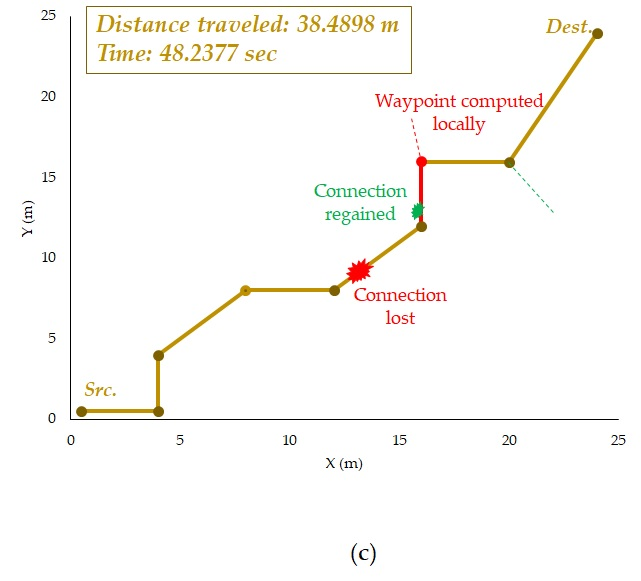
\includegraphics[width=2.5in,height=2.5in]{pf_c.jpg}
 \caption{Waypoint generation: (c) a scenario where both cloud and on-board resources are involved due to connectivity loss  \label{fig:PF_C}}
\end{figure}

Figure \ref{fig:PF_D_E} (d) shows a scenario where a request is originally forwarded to the cloud but the response hasn’t been received on time (say, due to temporary cloud resource outage). In this case, the timeout value for the request expires and the resource selector would choose to forward the request to the local resource (Note: here the timeout value is chosen based on the latency requirement to receive next waypoint specified in the Control Application Specification component in the offloading controller). Once the next waypoint from the cloud is received (after a large delay), the robotic controller would update its intermediate goal and starts moving towards that direction. 

\begin{figure}
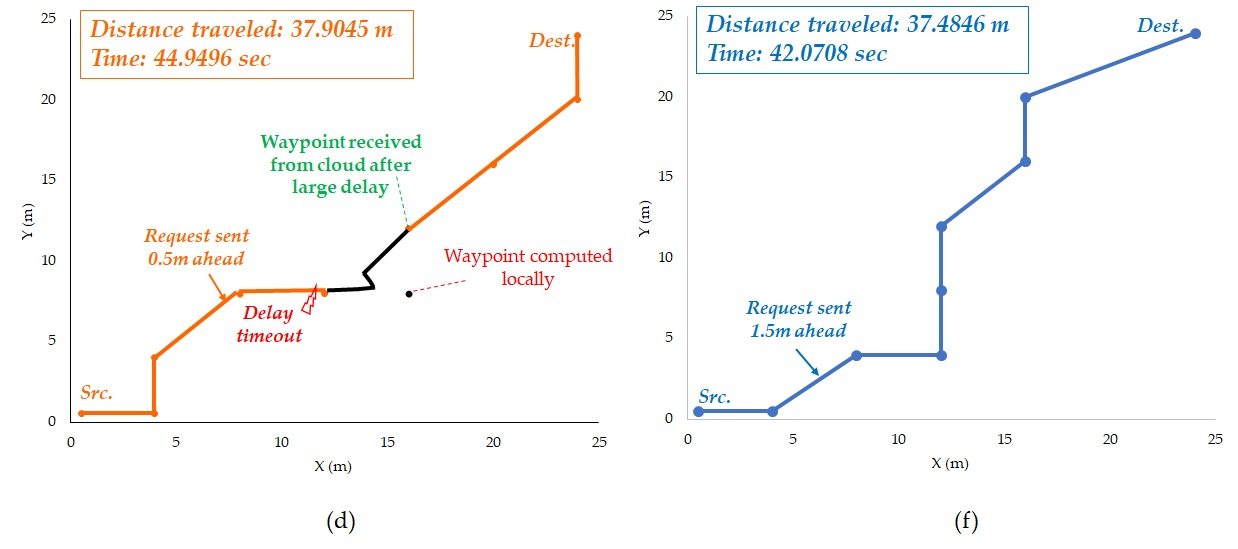
\includegraphics[width=3.5in,height=2.5in]{pf_d_e.jpg}
 \caption{Waypoint generation:  (d) a scenario where both cloud and on-board resources are involved due to large delay; (e) overcome transient large delays by requesting ahead of time  \label{fig:PF_D_E}}
\end{figure}

In Figure \ref{fig:PF_D_E} (d), the request for next waypoint is sent when the robot is 0.5 m ahead of the intermediate goal. One way to overcome large delay is to increase the distance at which the request for next waypoint is sent to the cloud. Figure \ref{fig:PF_D_E} (e) shows the performance results when the request is sent 1.5 m ahead of intermediate goal (as against 0.5 m ahead).

In this section, we have shown that a cloud-based path following controller improves the performance of the system compared a fully local resource based controller. Also, we have demonstrated the feasibility of switching between local and remote resources that effectively results in stable performance of the system despite a minor performance degradation.

\section{Related Work}
\label{sec:related.date17}
A few research groups in academia considered cloud-based automotive control applications and developed prototype models involving cloud. One such work, called Carcel \cite{ref:cloud_mit}, involves development of a cloud-assisted system for obstacle detection and avoidance for efficient path planning for autonomous vehicles. The system uses infrastructure sensor data in addition to in-vehicle data to sense obstacles ahead of time. The results reported in this work show a better reaction time to obstacles compared to a non-cloud-based collision avoidance system. A survey of decision making problems in self-driving cars with a focus on motion planning is presented in \cite{ref:motionplan_survey}. Motion planning involve computing dynamically feasible trajectory computation for a given source and destination pair. This survey presents different approaches to planning and their computational complexity.

A declarative approach to detect dangerous events by combining vehicle sensor data and static road information obtained from a cloud database is proposed in \cite{ref:carlog}. The declarative rules are defined using a sensor predicate and a cloud predicate. A cloud-based vehicle location tracking approach for urban environments, called CARLOC, is proposed in \cite{ref:carloc}. GPS systems have typically poor accuracy in urban environments. A probabilistic position that uses odometer, vehicle heading direction information from the vehicle and an online map database and landmark information is used to achieve lane level accuracy in determining the location of a vehicle. 

A software architecture for cloud-based automotive control is proposed in \cite{ref:caas}. The proposed futuristic approach involve only sense and actuate functions in the physical world whereas the control computations are preformed entirely in the cloud. This would enable offering Control as a Service (CaaS). The vehicle owners can customize and access control as a service on-demand from the cloud under the pay-per-use model. An architecture for cloud-based remote vehicle diagnostics, called AutoPlug, is proposed in \cite{ref:car_cloud}. The proposed architecture would enable proactively detecting software faults using diagnostic trouble codes, and allow code updates to be dispatched from a remote datacenter to vehicle electronic control units.

In contrast with the works cited above, our work aims to arrive at a generic approach to leverage cloud for control applications based on computational resource/data availability. Our approach also factors in varying communication link conditions (such as path loss and large delays) and allows dynamically switching between local and cloud resources. This ensures stability of the control system, although the control application performance may be less efficient in a local-only computation/data approach.
\section{Conclusion}
\label{sec:concl}
Cloud computing (and other remote computing technology variants such as fog or edge computing) is gaining traction in the automotive domain. To enhance in-vehicle and fault tolerance capabilities of self-driving vehicles, critical control applications can leverage such technologies. In this work, we presented our envisaged offloading controller design that would enable realization of remote resource based control applications. Using a cloud-based path following controller case study, we had demonstrated the feasibility of our approach in the presence of hostile network conditions. 
In the future, this work can be extended to study a more comprehensive control application and quality metrics that would allow us to perform a detailed trade-off analysis between the fully local computation and remote computation approaches. In addition, more hostile network conditions such as packet loss, corrupted packet can be simulated using NS-3 and interfaced with Matlab.



\bibliographystyle{unsrt}
\bibliography{DATE17_bibl}

\end{document}
